% JFM Rapids draft: Capillary effects on the self-similar growth of immiscible Rayleigh--Taylor mixing
% Figures: ../figures/fig_*.pdf, generated by ../make_figures.ipynb. Bibliography: jfm.bib.
% Class: jfm.cls + jfm.bst from the authors' (Overleaf) template. Rapids limit: 10 pages with the unmodified class, including figures and references.

\documentclass[lineno]{jfm}

\usepackage{graphicx}
\graphicspath{{../figures/}}
\usepackage{newtxtext}
\usepackage{newtxmath}
\usepackage{natbib}
\usepackage{stmaryrd}
\usepackage{hyperref}
\hypersetup{
    colorlinks = true,
    urlcolor   = blue,
    citecolor  = black,
}

% notation
\newcommand{\avg}[1]{\langle #1\rangle}
\newcommand{\At}{\mathrm{A_t}}
\newcommand{\We}{\mathrm{We}_0}
\newcommand{\lls}{\ell_\sigma}
\newcommand{\hd}{\dot h}
\newcommand{\pd}[2]{\frac{\partial #1}{\partial #2}}

\title{Capillary effects on the self-similar growth of immiscible Rayleigh--Taylor mixing}

\author{Michael D. Walker\aff{1}
  \corresp{\email{michael.walker@princeton.edu}}
 \and Stefan S. Nixon\aff{2}}

\affiliation{\aff{1}Department of Mechanical and Aerospace Engineering, Princeton University, Princeton, NJ 08544, USA
\aff{2}Department of Aeronautics, Imperial College London, London SW7 2AZ, UK}

\begin{document}
\maketitle

\begin{abstract}
In immiscible Rayleigh--Taylor turbulence, the growth parameter $\alpha$ increases as the initial Weber number $\We$ decreases, approximately as $\We^{-1/2}$ in recent simulations. This paper derives the form that such a dependence can take in a self-similar mixing layer. Complete self-similarity leaves no dimensionless group containing the surface tension, so $\We$ can enter only through corrections in the ratio of the capillary length $\lls$ to the layer width $h$. When the self-similar moment analysis of Ristorcelli \& Clark (\textit{J.~Fluid Mech.}, vol.~507, 2004, p.~213) is extended to immiscible fluids, the direct capillary term in the mid-plane scalar-flux budget is the inverse instantaneous Weber number, $(\lls/h)^2/2 \alpha$; it reduces $\alpha$ in proportion to $\We^{-1}$. With fixed profile constants, the same budget relaxes from any departure approximately as $h^{-40}$, so an increase that decays slowly with $h$ requires an indirect effect of surface tension on the flow structure. A correction linear in $\lls/h$ gives $\alpha - \alpha_\infty \propto \We^{-1/2}$ at fixed $h/\lambda_0$, and a spectral closure in which surface tension sets the inner cut-off of a smooth interface produces this form. High-resolution simulations compared at equal mixing width support the form $\alpha - \alpha_{\We = \infty} \approx 8.9 \, \lls/h$, whereas exponents extracted at fixed time drift with the time of comparison.
\end{abstract}

\begin{keywords}
buoyancy-driven instability, turbulent mixing, multiphase flow
\end{keywords}

% {\bf MSC Codes }  {\it(Optional)} Please enter your MSC Codes here

%=====================================================================
\section{Introduction}\label{sec:intro}

The late-time growth of a Rayleigh--Taylor (RT) mixing layer is usually written in the form of the constant-acceleration ansatz $h \approx \alpha \At g t^2$, where $h$ is the layer width, $g$ the acceleration, $\At$ the Atwood number and $\alpha$ a growth parameter that depends on the initial conditions \citep{Youngs1984,Dimonte2004}. \citet{Ristorcelli2004} (hereafter RC04) showed that self-similarity of the second-moment equations gives $\hd^2 = \At g C_\mathrm{o} h$, so that $\alpha = C_\mathrm{o}/4$ is a functional of the unclosed self-similar profiles rather than a universal constant. Immiscible fluids grow faster. Experiments, many of them with immiscible fluids, give larger $\alpha$ than simulations of miscible mixing \citep{Dimonte2000,Dimonte2004}, and at $\At \approx 0.5$ miscibility reduced $\alpha$ by about a factor of two in direct comparisons \citep{Roberts2016}. \citet{Cook2004} (hereafter CCM04) argued from the mid-plane mass flux, where density fluctuations take their largest possible value, that immiscible fluids should grow faster, and recent incompressible, low-order volume-of-fluid simulations find $\alpha$ increasing with surface tension \citep{Zhao2026_1,Zhao2026_2}.

Compressible, high-order diffuse-interface simulations at $\At = 0.5$ \citep{Brill2025,Walker2025,Walker2026,Walker2027_1} give $\alpha \approx 0.039$ for immiscible fluids without surface tension and $\alpha \approx 0.028$ for miscible fluids, and a further increase as the initial Weber number $\We$ decreases (figure~\ref{fig:alpha}\textit{a}). The trend was reported as approximately $\alpha \propto \We^{-1/2}$ on dimensional grounds \citep{Walker2026}. Linear theory predicts the opposite tendency, since surface tension stabilises short wavelengths \citep{Chandrasekhar_book,Sohn2009}. This paper derives the form that a $\We$ dependence can take in a self-similar layer, by extending the RC04 analysis to immiscible fluids with surface tension, and compares it with the simulations at equal mixing width.

\begin{figure}
  \centering
  \begin{minipage}[t]{0.49\textwidth}\raggedright (\textit{a})\\[-2pt]
    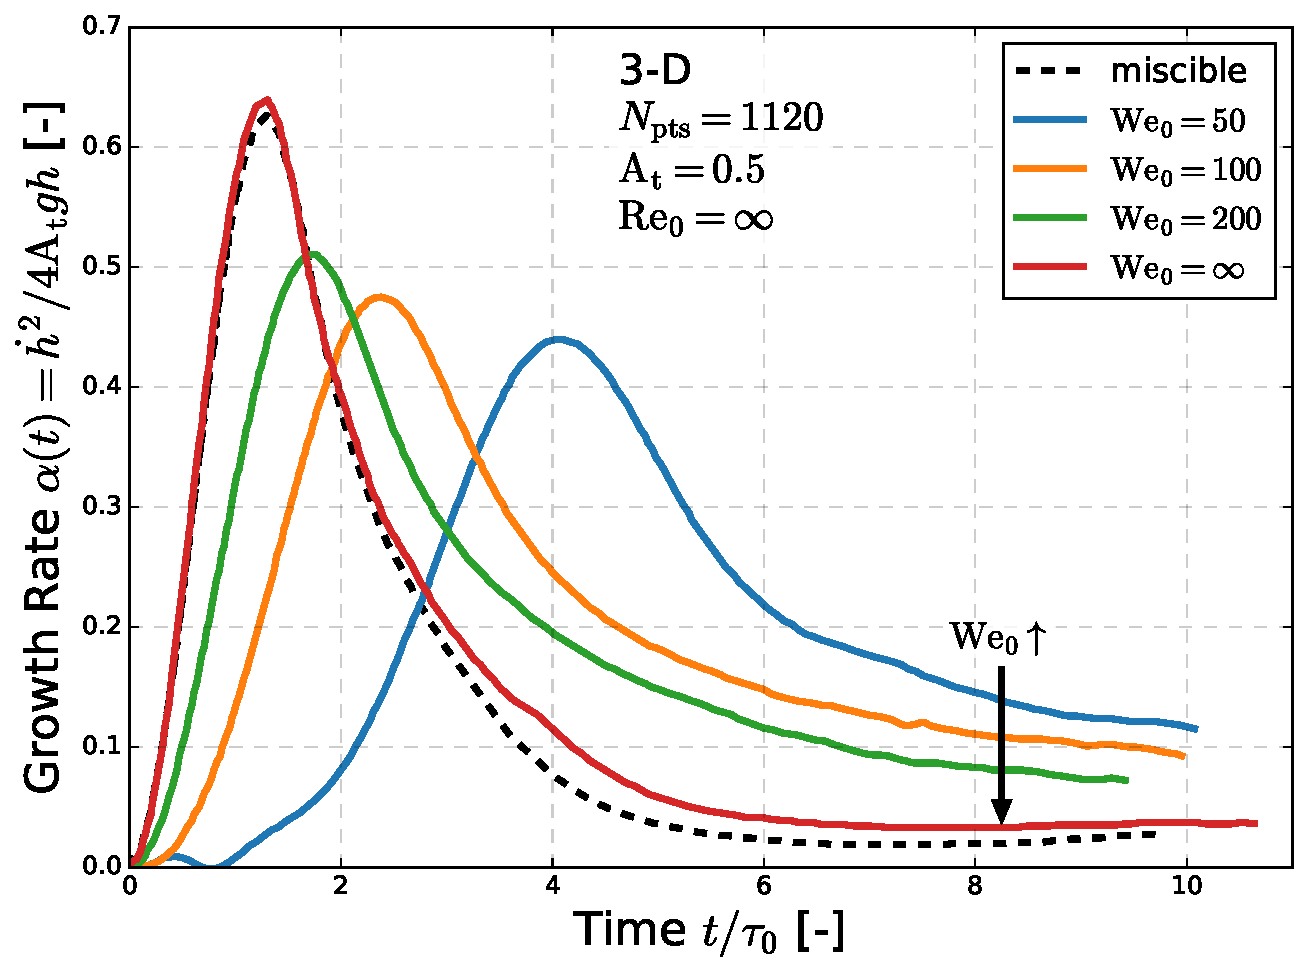
\includegraphics[width=\linewidth]{fig_alpha_time}\end{minipage}\hfill
  \begin{minipage}[t]{0.505\textwidth}\raggedright (\textit{b})\\[-2pt]
    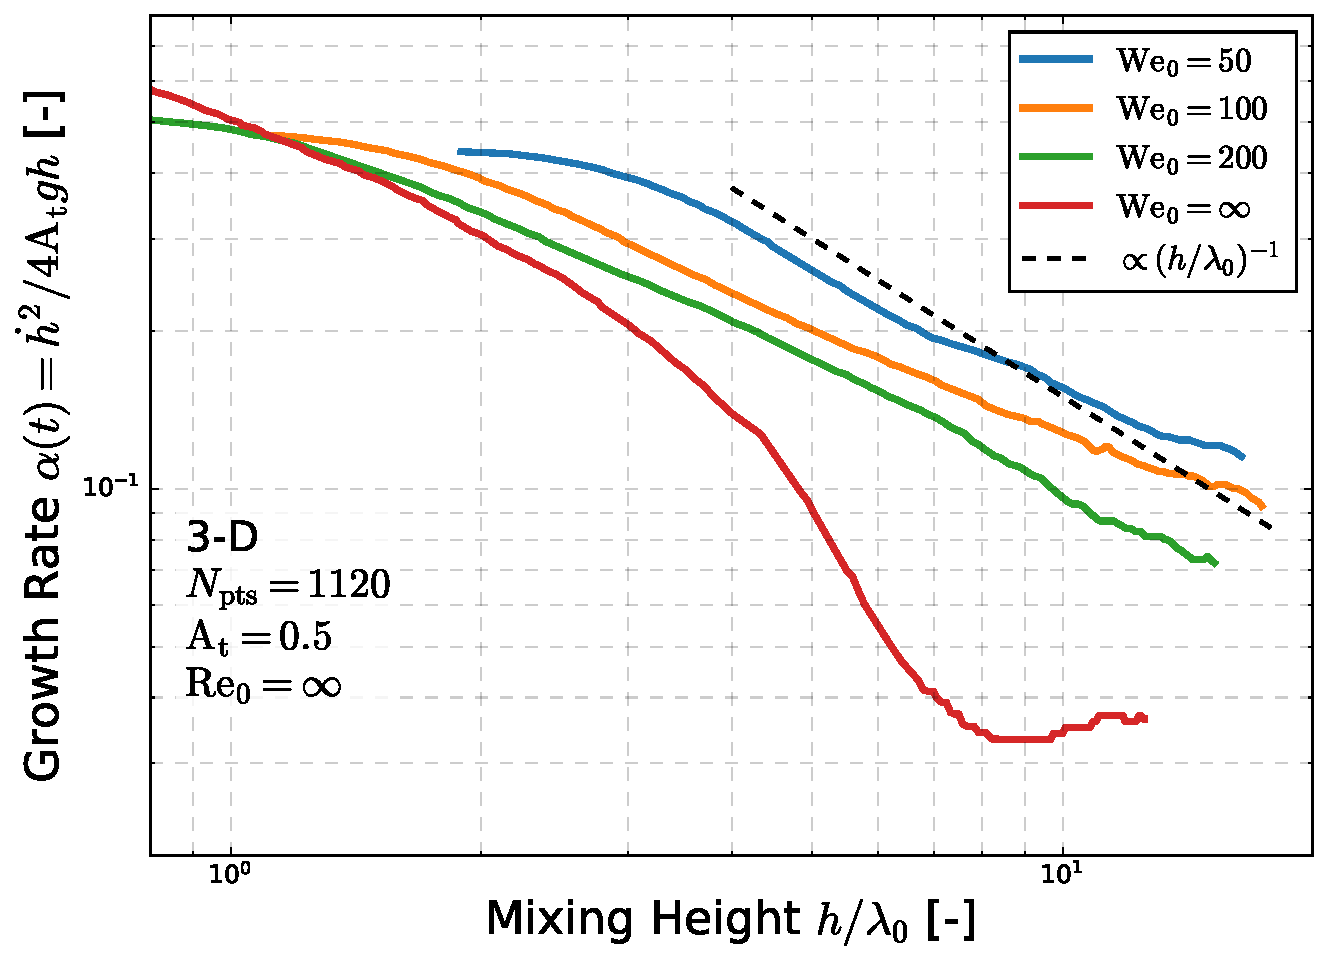
\includegraphics[width=\linewidth]{fig_alpha_height}\end{minipage}
  \caption{Growth parameter $\alpha(t) = \hd^2/4 \At g h$ in the immiscible simulations of \citet{Walker2025,Walker2026,Walker2027_1} at $\We = 50$, $100$, $200$ and $\infty$, with $1120^3$ points, $\At = 0.5$ and $\mathrm{Re}_0 = \infty$: (\textit{a}) against $t/\tau_0$, with a miscible simulation for reference; (\textit{b}) against $h/\lambda_0$ after the peak of $\alpha$, on logarithmic axes.}
  \label{fig:alpha}
\end{figure}

%=====================================================================
\section{Constraints from dimensional analysis}\label{sec:dim}

Two fluids of densities $\rho_h > \rho_\ell$, separated by an interface with surface tension coefficient $\sigma$, are accelerated by gravity $g$ in the $-z$ direction. With $\bar\rho = (\rho_h + \rho_\ell)/2$, $\Delta \rho = \rho_h - \rho_\ell$ and $\At = \Delta \rho/2 \bar\rho$, an initial perturbation of shortest wavelength $\lambda_0$ defines $\tau_0 = (\lambda_0/\At g)^{1/2}$ and
\begin{equation}
  \We = \frac{\bar\rho \, g \, \lambda_0^2}{\sigma} \, , \qquad \lls = \Big(\frac{\sigma}{\Delta \rho \, g}\Big)^{1/2} \, , \qquad \frac{\lls}{\lambda_0} = (2 \At \We)^{-1/2} \;,
  \label{eq:params}
\end{equation}
where $\lls$ is the cut-off length of linear theory, $\gamma^2 = \At g k \,(1 - k^2 \lls^2)$ \citep{Chandrasekhar_book,Sohn2009}. The width is the full width $h = 6 \int \bar V(1 - \bar V) \, \mathrm d z$, which equals the total width of a linear profile, with $\bar V$ the plane-averaged volume fraction of heavy fluid, and the growth parameter is measured instantaneously as $\alpha(t) = \hd^2/4 \At g h$, which is constant for the RC04 solution with its virtual origin. Dimensional analysis gives $\alpha = \Psi(t/\tau_0; \At, \We, \mathrm{Re}_0, \dots)$ and admits any dependence on $\We$. The quantities $\sigma/\bar\rho$ and $\At g$ define the length $\lls$ but no dimensionless group, so a second length is needed. Under complete self-similarity, the only one available is $h$, the initial wavelength is forgotten, and the relevant group is the instantaneous Weber number
\begin{equation}
  \mathrm{We}(t) \equiv \frac{\bar\rho \, \hd^2 h}{\sigma} = 4 \At \, \alpha \, \We \Big(\frac{h}{\lambda_0}\Big)^2 \, , \qquad \Big(\frac{\lls}{h}\Big)^2 = \frac{2 \alpha}{\mathrm{We}(t)} \;,
  \label{eq:We_t}
\end{equation}
which grows as $t^4$. If a self-similar state exists with $h$ as its only outer length, $\alpha$ tends to a limit $\alpha_\infty$ independent of $\sigma$, and a $\We$ dependence survives only as a correction in $\lls/h$ that decays as the layer grows, an incomplete similarity in the sense of \citet{Barenblatt1996}. A persistent power law in $\We$ is excluded. One such correction follows from a velocity scale set by capillarity and buoyancy alone, $U_\sigma \propto (\At g \lls)^{1/2}$. Adding $U_\sigma^2$ to the self-similar $\hd^2 = 4 \alpha_\infty \At g h$ gives
\begin{equation}
  \alpha(t) = \alpha_\infty + K \, \frac{\lls}{h} = \alpha_\infty + K \,(2 \At \We)^{-1/2} \, \frac{\lambda_0}{h} \;,
  \label{eq:capvel}
\end{equation}
with $K$ a constant. This is the form in which a $\We^{-1/2}$ dependence is consistent with dimensional analysis: at fixed $h/\lambda_0$, as a correction that decays as $h^{-1}$. A power law $\alpha \propto \We^{-1/2}$ would give $\alpha \rightarrowtriangle 0$ as $\sigma \rightarrowtriangle 0$, contrary to $\alpha \approx 0.039$ at $\We = \infty$.

%=====================================================================
\section{Mid-plane scalar-flux budget}\label{sec:flux}

Following RC04, this approach begins with the Boussinesq form. Let $c = +1$ in the heavy fluid and $c = -1$ in the light fluid, so that $\rho = \bar\rho(1 + \At c)$. Let $\mathbf u = (u, v, w)$ be the velocity, $\mu$ the dynamic viscosity, $p$ the kinematic pressure (pressure divided by $\bar\rho$), and $\mathbf f = (\sigma/\bar\rho) \, \kappa \, \hat{\mathbf n} \, \delta_s$ the capillary force per unit mass \citep{Brackbill1992}, with $\hat{\mathbf n} = \nabla c/| \nabla c |$, curvature $\kappa = -\nabla \cdot \hat{\mathbf n}$ and $\delta_s$ the surface delta function. Angle brackets denote averages over horizontal planes, $c = C + c'$ with $C = \avg c$, and the subscript `$0$' denotes the mid-plane $z = 0$. Because $c^2 = 1$ everywhere,
\begin{equation}
  \avg{c' c'} = 1 - C^2 \;,
  \label{eq:constraint}
\end{equation}
so the molecular mixing parameter of RC04 vanishes, the scalar-variance equation is satisfied, and $\avg{c' c'}_0 = 1$; for miscible fluids, $\avg{c' c'}_0 = 1 - \theta_0$, with $\theta_0$ the mixedness. Integrating the mean indicator equation from $-\infty$ to the mid-plane with the self-similar profile $C = f_C(z/h)$ gives $\avg{w c'}_0 = -2 \hd/R_f$ (\S\,S1 of the supplementary material), where $R_f = \Delta \rho \, \hd/| \avg{\rho' w'}_0 |$ depends, for a self-similar layer, only on the shape of $\bar V$; it is $8.0$--$8.7$ for linear, error-function and hyperbolic-tangent profiles. The scalar-flux equation (RC04, their equation 2.8) with surface tension is
\begin{equation}
  \pd{}{t} \avg{w c'} + \pd{}{z} \avg{w w c'} = -\avg{w w} \pd{C}{z} - \At g \avg{c' c'} - \Big\langle c' \pd{p}{z} \Big\rangle + \avg{c' f_z} + \frac{\mu}{\bar\rho} \avg{c' \nabla^2 w} \;.
  \label{eq:flux}
\end{equation}
Taking the divergence of the momentum equation gives a Poisson equation for the pressure fluctuation $p'$,
\begin{equation}
  \nabla^2 p' = -\At g \, \pd{c'}{z} - \frac{\partial^2 (u_i u_j - \avg{u_i u_j})}{\partial x_i \, \partial x_j} + \nabla \cdot (\mathbf f - \avg{\mathbf f}) \;,
  \label{eq:poisson}
\end{equation}
where $u_i$ and $x_i$ are the velocity and position components. Because (\ref{eq:poisson}) is linear, $p'$ splits into buoyancy, nonlinear and capillary parts, $p' = p_B + p_N + p_\sigma$, each driven by one of the three source terms. The buoyancy part is set by the indicator field alone, $p_B = -\At g \, \nabla^{-2} (\partial c'/\partial z)$, where $\nabla^{-2}$ is the inverse Laplacian, and it opposes the force that drives it: a heavy parcel raises the pressure in the fluid below it, which pushes back against its descent. Its contribution to the pressure--scalar correlation in (\ref{eq:flux}) is therefore proportional to the buoyancy production itself,
\begin{equation}
  -\At g \avg{c' c'} - \Big\langle c' \pd{p_B}{z} \Big\rangle = -\At g \,(1 - \chi) \avg{c' c'} \, , \qquad \chi \equiv \frac{1}{\avg{c' c'}} \Big\langle c' \, \frac{\partial^2}{\partial z^2} \nabla^{-2} c' \Big\rangle \;,
  \label{eq:chi}
\end{equation}
so the buoyancy pressure cancels a fraction $\chi$ of the buoyancy production. For a statistically homogeneous field with Fourier coefficients $\hat c_{\mathbf k}$, $\chi = \sum_{\mathbf k} (k_z^2/k^2) | \hat c_{\mathbf k} |^2 / \sum_{\mathbf k} | \hat c_{\mathbf k} |^2$ is the fraction of the indicator variance at vertical wavenumbers. It depends only on the shape of the structures: $\chi = 0$ for vertical columns, which slide past one another without a pressure response; $\chi = 1/3$ for isotropic structures; and $\chi \rightarrowtriangle 1$ for horizontal layers, whose weight is carried entirely by the pressure. In the same way, the capillary pressure removes the gradient part of the capillary force. The two capillary terms in (\ref{eq:flux}) combine into $\avg{c' (\mathcal P \mathbf f)_z}$, where $\mathcal P \mathbf f = \mathbf f - \avg{\mathbf f} - \nabla p_\sigma$ and $\mathcal P$ is the projection onto divergence-free fields (the Leray--Helmholtz projection). The Laplace pressure of a drop in equilibrium is a pure gradient, which $\mathcal P$ removes, so only the part of the capillary force that can drive a flow enters the budget. Let $d_T$, $d_N$, $d_\mu$ and $d_\sigma$ denote the mid-plane turbulent-transport, nonlinear-pressure, viscous and capillary terms, normalised by $\hd^2/h$ and signed so that a positive value is a sink of $-\avg{w c'}_0$. On the mid-plane, (\ref{eq:flux}) becomes an ordinary differential equation for $h$,
\begin{align}
\frac{2}{R_f} \, \ddot h = \At g \,(1 - \chi_0) \avg{c' c'}_0 - &\Big(\hat D - \frac{1}{R_f} + d_\sigma\Big) \frac{\hd^2}{h} \,, \nonumber \\ \hat D & = \frac{1}{R_f} + d_T + d_N + d_\mu - \hat w \, f_C'(0) \;, \label{eq:ode}
\end{align}
with $\hat w = \avg{w w}_0/\hd^2$ and $f_C'(0) = h \, \partial C/\partial z |_0$. For $\hd^2 \propto h$, $\ddot h = \hd^2/2 h$ and
\begin{equation}
  \hd^2 = \At g \, h \, \frac{\avg{c' c'}_0 \,(1 - \chi_0)}{\hat D + d_\sigma} \, , \qquad C_\mathrm{o} \equiv \frac{\avg{c' c'}_0 \,(1 - \chi_0)}{\hat D} = 4 \alpha_\infty \;.
  \label{eq:alpha}
\end{equation}
Without surface tension, this is the RC04 result $\hd^2 = \At g C_\mathrm{o} h$, with the constant written as mid-plane statistics: a purity $\avg{c' c'}_0$, which is unity for immiscible fluids, a buoyancy efficiency $1 - \chi_0$, and a normalised inertia and drag $\hat D$.

%=====================================================================
\section{Direct effect of surface tension}\label{sec:direct}

In RC04, every energy-containing quantity scales with $h$. The curvature and the interface area per unit volume that contribute to $\avg{c' (\mathcal P \mathbf f)_z}$ then scale as $1/h$, and the capillary group is the inverse instantaneous Weber number,
\begin{equation}
  d_\sigma \sim \frac{\sigma}{\bar\rho \, h \, \hd^2} = \frac{1}{\mathrm{We}(t)} = \frac{1}{2 \alpha} \Big(\frac{\lls}{h}\Big)^2 \;.
  \label{eq:dsigma}
\end{equation}
Writing $d_\sigma = \hat d_\sigma (\lls/h)^2$ and expanding (\ref{eq:alpha}) for $d_\sigma \ll \hat D$ (\S\,S2 of the supplementary material),
\begin{equation}
  \alpha(t) = \alpha_\infty \Big[1 - a_\sigma \Big(\frac{\lls}{h}\Big)^2\Big] = \alpha_\infty \Big[1 - \frac{a_\sigma}{2 \At \We} \Big(\frac{\lambda_0}{h}\Big)^2\Big] \, , \qquad a_\sigma = \frac{\hat d_\sigma}{\hat D} > 0 \;.
  \label{eq:direct}
\end{equation}
The sign follows from the restoring character of the capillary force: at the tip of a falling spike, where $c' > 0$, it points upward, and at the cap of a rising bubble, where $c' < 0$, it points downward, so $c' f_z > 0$ and $d_\sigma > 0$. The direct effect of surface tension is therefore a correction proportional to $\We^{-1}$ that decays as $h^{-2}$ and reduces $\alpha$. At the end of the simulations of \citet{Walker2025,Walker2026,Walker2027_1} (see \S\,\ref{sec:sims}), $\mathrm{We}(t) \approx (3$--$7) \times 10^3$ (figure~\ref{fig:theory}\textit{a}), so $d_\sigma \sim 10^{-4}$ while $\hat D = \mathcal{O}(1)$.

Small-scale interfacial structure does not change this conclusion. Turbulence should be unable to deform the interface at scales below the Hinze scale $\ell_H$ \citep{Kolmogorov1949,Hinze1955}. With the inviscid dissipation scaling of RC04, $\varepsilon_0 = C_\varepsilon \hd^3/h$, and $\hd^2 = 4 \alpha \At g h$,
\begin{equation}
  \ell_H = C_H \Big(\frac{\sigma}{\bar\rho}\Big)^{3/5} \varepsilon^{-2/5} \, , \qquad \frac{\ell_H}{h} = K_H \Big(\frac{\lls}{h}\Big)^{6/5} \, , \qquad K_H = C_H \, C_\varepsilon^{-2/5} (2 \alpha)^{-3/5} \;,
  \label{eq:hinze}
\end{equation}
with $C_H \approx 0.725$, so that $K_H \approx 3.3$ for $\alpha = 0.04$ and $C_\varepsilon = 1$. The Hinze scale therefore also separates from $h$ as the layer grows \citep{Chertkov2005}, and the capillary force on structures near $\ell_H$ is balanced mainly by Laplace pressure. The Hinze scale evaluated with the dissipation rate of the simulations \citep{Walker2027_2} follows this scaling (figure~S1 of the supplementary material). For $6 \le t/\tau_0 \le 9.4$, it decreases as $h^{-0.11}$ to $h^{-0.35}$ for the three Weber numbers, around the $h^{-1/5}$ of (\ref{eq:hinze}), and a fit with that slope gives $K_H \approx 2.3$; with the late-time values of $\alpha$ in the simulations, $0.08$--$0.13$ rather than $0.04$, (\ref{eq:hinze}) gives $K_H \approx 1.6$--$2.2$. At $t = 9.4 \tau_0$, $\ell_H/\lls \approx 0.8$--$0.9$ and $\ell_H \approx 0.6$--$1.1$ times the grid spacing, so the Hinze scale, the capillary length and the grid spacing are comparable. Across Weber numbers, $\ell_H$ varies as $\We^{-0.45}$ rather than $\We^{-3/5}$, so the dissipation rate also depends on $\We$. The capillary term can instead be estimated at $\ell_H$, as the ratio of capillary to buoyancy pressure at that scale weighted by the relative amplitude of the indicator fluctuation there. If the second-order structure function of the indicator scales as $r^{2 q}$ (\S\,\ref{sec:closure}), (\ref{eq:hinze}) gives
\begin{equation}
  \frac{\sigma/\ell_H}{\Delta \rho \, g \, \ell_H} \Big(\frac{\ell_H}{h}\Big)^{q} = \Big(\frac{\lls}{\ell_H}\Big)^2 \Big(\frac{\ell_H}{h}\Big)^{q} \propto \Big(\frac{\lls}{h}\Big)^{\nu} \, , \qquad \nu = \frac{6 q - 2}{5} = \frac{7 - 3 D_s}{5} \;,
  \label{eq:hinze_estimate}
\end{equation}
where $D_s$ is the fractal dimension of the interface. For $D_s \ge 2$, the exponent is at most $1/5$; for the values $D_s \approx 2.6$--$2.7$ reported for scalar iso-surfaces in turbulence \citep{Sreenivasan1991}, it is negative, and the correction would grow with $h$. The sign is again restoring.

\begin{figure}
  \centering
  \begin{minipage}[t]{0.50\textwidth}\raggedright (\textit{a})\\[-2pt]
    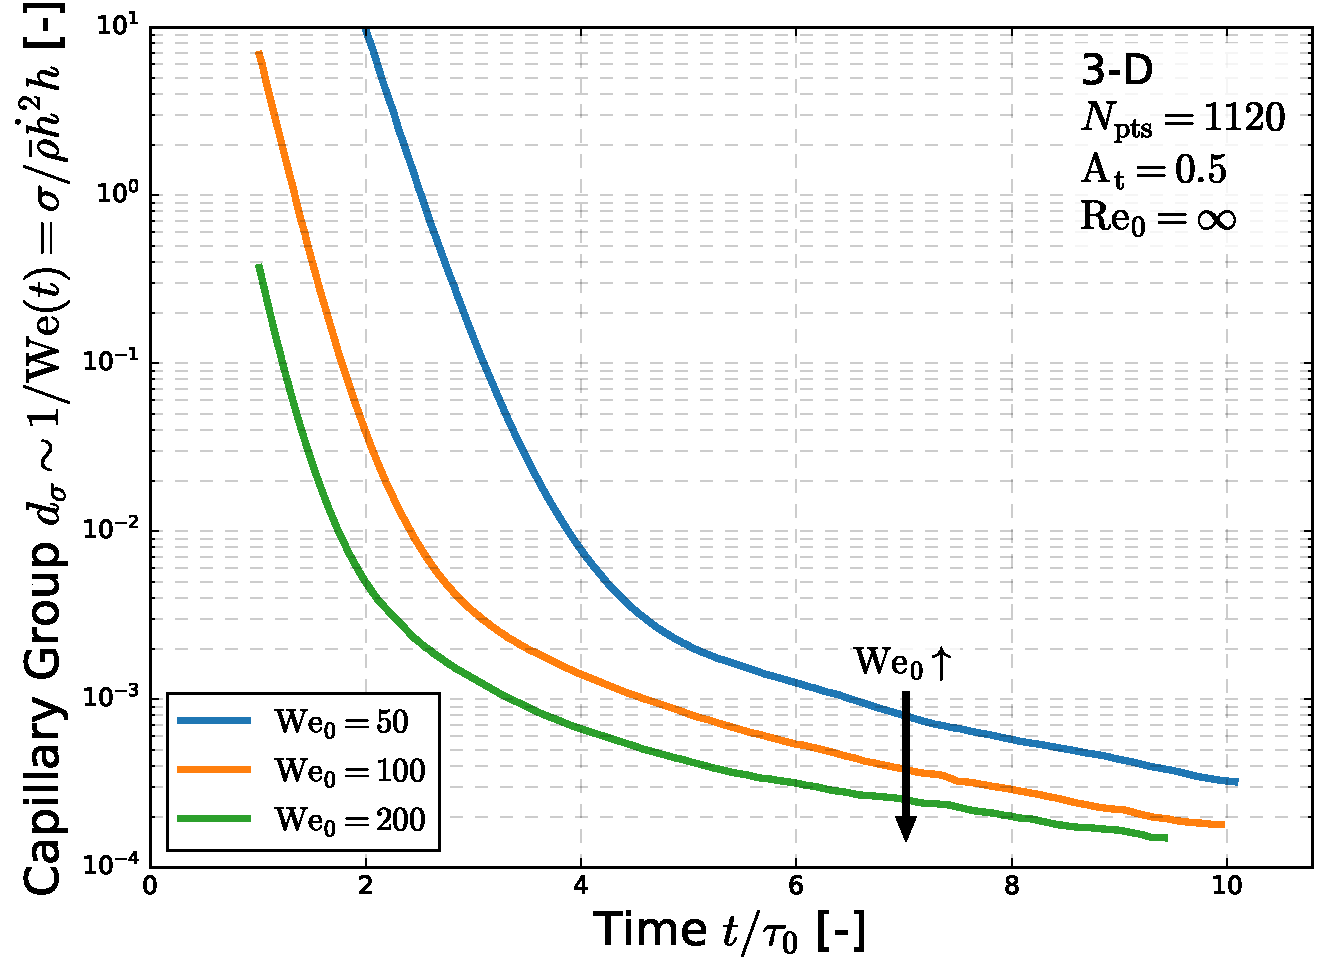
\includegraphics[width=\linewidth]{fig_capillary_group}\end{minipage}\hfill
  \begin{minipage}[t]{0.495\textwidth}\raggedright (\textit{b})\\[-2pt]
    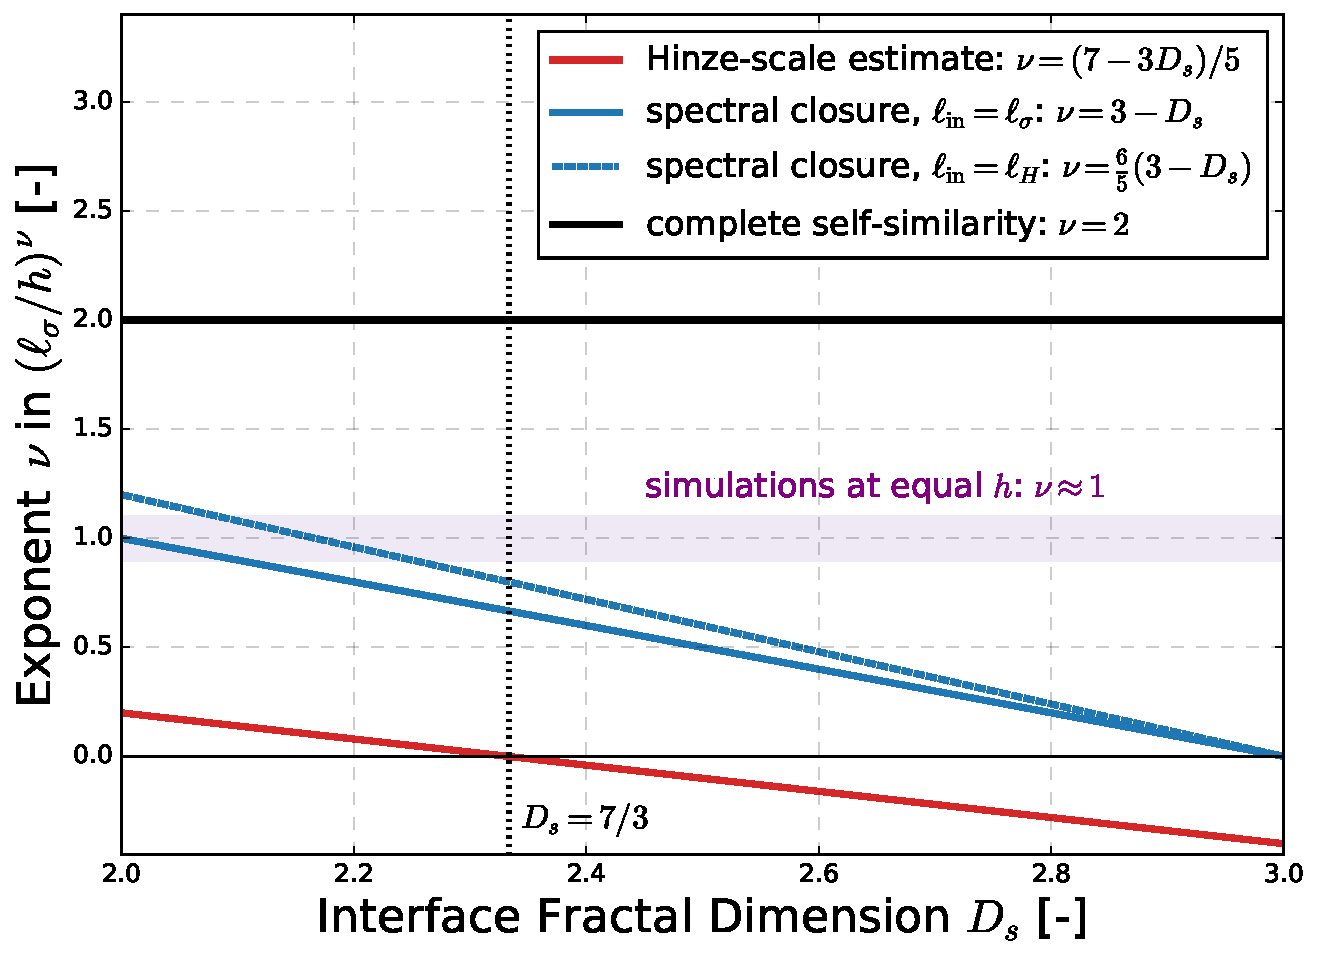
\includegraphics[width=\linewidth]{fig_nu_Ds}\end{minipage}
  \caption{(\textit{a}) Capillary group $d_\sigma \sim 1/\mathrm{We}(t)$, (\ref{eq:dsigma}), in the simulations of \citet{Walker2025,Walker2026,Walker2027_1} at $\We = 50$, $100$ and $200$. (\textit{b}) Exponent $\nu$ of the correction $(\lls/h)^{\nu}$ against the interface fractal dimension $D_s$: complete self-similarity, (\ref{eq:direct}); the Hinze-scale estimate, (\ref{eq:hinze_estimate}); and the spectral closure, (\ref{eq:We_scaling}), with $\ell_{\rm in} = \lls$ and $\ell_{\rm in} = \ell_H$. The shaded band marks $\nu \approx 1$ from the simulations at equal mixing width.}
  \label{fig:theory}
\end{figure}

%=====================================================================
\section{Relaxation towards self-similarity}\label{sec:relax}

Equation (\ref{eq:ode}) also describes how a departure from $\hd^2 \propto h$ decays when the profile constants are fixed. Writing $y = \hd^2$, so $\ddot h = \tfrac12 \, \mathrm d y/\mathrm d h$, and setting $d_\sigma = 0$,
\begin{equation}
  \frac{\mathrm d y}{\mathrm d h} + (R_f \hat D - 1) \, \frac{y}{h} = R_f \At g \,(1 - \chi_0) \avg{c' c'}_0 \;, \qquad \mbox{so that} \qquad \alpha(t) - \alpha_\infty \propto h^{-R_f \hat D} \;.
  \label{eq:relax}
\end{equation}
With $\alpha_\infty \approx 0.035$, $\chi_0 \approx 1/3$ and $R_f \approx 8.0$, the values without surface tension, (\ref{eq:alpha}) gives $\hat D \approx 4.8$ and $R_f \hat D \approx 40$. Departures from self-similar growth therefore decay as a high power of $h$, and a correction that decays as $h^{-1}$, such as (\ref{eq:capvel}), cannot be a transient of the moment balance with fixed constants. Together with the sign of (\ref{eq:direct}), this shows that an increase of $\alpha$ with $\sigma$ requires an indirect effect of surface tension on the flow structure: either a slow evolution of $\chi_0$ and $\hat D$ with $h$, or an additional term in the balance that scales as $\lls/h$. If surface tension instead fixed the profile constants during the transition, when $\lls/\lambda_0$ is not small, $\alpha_\infty$ itself would depend on $\We$ and the excess would not decay with $h$.

%=====================================================================
\section{A spectral closure}\label{sec:closure}

The inner cut-off of the indicator spectrum provides an indirect effect of the required form (\S\,S4 of the supplementary material). For a two-phase indicator, the second-order structure function $\avg{[c(\mathbf x + \mathbf r) - c(\mathbf x)]^2}$ is proportional to the probability that a segment of length $r$ crosses the interface. That probability scales with the interface area per unit volume measured at resolution $r$, which is proportional to $h^{-1}(h/r)^{D_s - 2}$, so the structure function scales as $r^{3 - D_s}$ \citep{Sreenivasan1991}. Defining $q$ by a structure function proportional to $r^{2 q}$ and $p$ by a spectrum $E_c(k) \propto k^{-p}$, with $p = 2 q + 1$,
\begin{equation}
  D_s = 3 - 2 q = 4 - p \;.
  \label{eq:pq}
\end{equation}
A smooth interface has $D_s = 2$ and the Porod spectrum $k^{-2}$ \citep{Porod1951}; an indicator with the Obukhov--Corrsin spectrum $k^{-5/3}$ \citep{Obukhov1949,Corrsin1951} has $D_s = 7/3$. Suppose that only the indicator variance at the energy-containing scales, $1/h \le k \le 2/h$, drives the energy-containing flux, the flux produced at small scales being destroyed locally as in the $k^{-7/3}$ range of the scalar-flux co-spectrum \citep{Lumley1967}. Replacing $\avg{c' c'}_0$ in (\ref{eq:alpha}) by that fraction of the variance, for a spectrum that extends from $1/h$ to an inner cut-off $1/\ell_{\rm in}$, gives
\begin{equation}
  \alpha(h) = \frac{\alpha_\infty}{1 - (\ell_{\rm in}/h)^{3 - D_s}} \approx \alpha_\infty \Big[1 + \Big(\frac{\ell_{\rm in}}{h}\Big)^{3 - D_s}\Big] \;.
  \label{eq:closure}
\end{equation}
Without surface tension, an immiscible indicator has no inner cut-off, $\ell_{\rm in} \rightarrowtriangle 0$. Surface tension sets $\ell_{\rm in}$ to the smaller of $\lls$, below which buoyancy cannot deform the interface, and $\ell_H$, below which turbulence cannot. By (\ref{eq:hinze}), $\ell_{\rm in} = \lls$ for $h/\lls \lesssim K_H^5$ and $\ell_{\rm in} = \ell_H$ beyond. In the simulations, $K_H^5 \approx 60$ and $h/\lls$ reaches $100$--$215$, so $\ell_H$ is slightly smaller than $\lls$ at late times; the two cut-offs differ by less than $25\,\%$ (figure~S1 of the supplementary material), and the simulations cannot distinguish the two branches of (\ref{eq:We_scaling}), which for $D_s = 2$ give $\nu = 1$ and $\nu = 6/5$. The correction (\ref{eq:closure}) increases $\alpha$ and, with (\ref{eq:params}) and (\ref{eq:hinze}),
\begin{equation}
  \frac{\alpha - \alpha_\infty}{\alpha_\infty} \approx
  \begin{cases}
  (2 \At \We)^{-(3 - D_s)/2} \, (\lambda_0/h)^{3 - D_s} \, , & h/\lls \lesssim K_H^5 \;, \\
  K_H^{3 - D_s} \,(2 \At \We)^{-3(3 - D_s)/5} \, (\lambda_0/h)^{6(3 - D_s)/5} \, , & h/\lls \gtrsim K_H^5 \;.
  \end{cases}
  \label{eq:We_scaling}
\end{equation}
For $D_s = 7/3$, this gives $\alpha - \alpha_\infty \propto \We^{-1/3}$ at fixed $h/\lambda_0$ in the intermediate regime and $\propto \We^{-2/5}$ asymptotically. A $\We^{-1/2}$ dependence requires $D_s = 2$ with $\ell_{\rm in} = \lls$, or $D_s = 13/6$ with $\ell_{\rm in} = \ell_H$. For a smooth interface with $\ell_{\rm in} = \lls$, (\ref{eq:We_scaling}) is (\ref{eq:capvel}) with $K = \alpha_\infty$: a correction linear in $\lls/h$, of the observed sign, and proportional to $\We^{-1/2}$ at fixed $h/\lambda_0$. Table~\ref{tab:compare} and figure~\ref{fig:theory}(\textit{b}) summarise the corrections.

\begin{table}
  \begin{center}
  \def~{\hphantom{0}}
  \small
  \begin{tabular}{p{0.21\textwidth}p{0.21\textwidth}llll}
    Origin & Basis & $\nu$ & Coefficient & $\We$ dependence & Effect $\sigma$ on $\alpha$ \\ \cline{1-6} \\[-9pt]
    Direct capillary term & \begin{tabular}{@{}l@{}} Moment equations, \\ Eq. (\ref{eq:direct}) \end{tabular} & $2$ & $-\alpha_\infty a_\sigma$ & $\propto -\We^{-1}$ & decrease\\
    Capillary term at $\ell_H$ & \begin{tabular}{@{}l@{}} Hinze-scale estimate, \\ Eq. (\ref{eq:hinze_estimate}) \end{tabular} & $(7 - 3 D_s)/5$ &  $\,$ --- & $\propto -\We^{-\nu/2}$ & decrease\\
    Inner cut-off $\ell_{\rm in} = \lls$ & \begin{tabular}{@{}l@{}} Spectral closure, \\ Eq. (\ref{eq:We_scaling}) \end{tabular} & $3 - D_s$ & $\alpha_\infty$ & $\propto \We^{-(3 - D_s)/2}$ & increase\\
    Inner cut-off $\ell_{\rm in} = \ell_H$ & \begin{tabular}{@{}l@{}} Spectral closure, \\ Eq. (\ref{eq:We_scaling}) \end{tabular} & $\tfrac65(3 - D_s)$ & $\alpha_\infty K_H^{3 - D_s}$ & $\propto \We^{-3(3 - D_s)/5}$ & increase\\
    Capillary velocity & \begin{tabular}{@{}l@{}} Dimensional analysis, \\ Eq. (\ref{eq:capvel}) \end{tabular} & $1$ & $K$ & $\propto \We^{-1/2}$ & increase\\
    Simulations, equal $h$ & \begin{tabular}{@{}l@{}} Fit, $7 \le h/\lambda_0 \le 12.5$, \\ Eq. (\ref{eq:fit}) \end{tabular} & $0.97$ & $8.9$ ($7.7$--$9.9$) & $\propto \We^{-1/2}$ & increase\\
    Simulations, fixed $t/\tau_0$ & Fit, $6 \le t/\tau_0 \le 9.4$ & --- & $\,$ --- & \begin{tabular}{@{}l@{}} $\alpha \propto \We^{-m}$, \\ $\; m = 0.37$--$0.46$ \end{tabular} & increase\\
  \end{tabular}
  \caption{Corrections to the growth parameter of the form $\alpha - \alpha_\infty = (\text{coefficient}) \times (\lls/h)^{\nu}$, and the resulting dependence on $\We$ at fixed $h/\lambda_0$.}
  \label{tab:compare}
  \end{center}
\end{table}

%=====================================================================
\section{Comparison with simulations}\label{sec:sims}

The simulations of \citet{Walker2025,Walker2026,Walker2027_1} solve the compressible multicomponent equations with the high-order compact finite-difference code \texttt{Miranda} \citep{Cook2007}, using localised artificial diffusivity with interface sharpening \citep{Brill2025} and a continuum surface force \citep{Brackbill1992}, on $1120^3$ points at $\At = 0.5$ and $\mathrm{Re}_0 = \infty$, for $\We = 50$, $100$, $200$ and $\infty$ and a miscible reference case; \citet{Walker2027_1} give the details. Decreasing $\We$ delays the transition, the time of maximum growth of the mixedness increasing linearly with $\sigma$ as $t_\theta/\tau_0 \approx 1.88 + 179/\We$ (\S\,S5 of the supplementary material), and raises the late-time $\alpha$ (figure~\ref{fig:alpha}\textit{a}).

Compared at fixed time, the effective exponent in $\alpha \propto \We^{-m}$, fitted over $\We = 50$, $100$ and $200$, drifts from $0.46$ at $t = 6 \tau_0$ to $0.37$--$0.38$ at $t = 8.5$--$9.4 \tau_0$ (figure~\ref{fig:excess}\textit{b} and table~S2 of the supplementary material), close at late times to the fit $\alpha \approx 0.49 \, \We^{-0.35}$ of \citet{Walker2026}. An exponent obtained at fixed time is therefore not a property of the flow; it depends on when the simulations are compared. The analysis above is formulated in $h$, and every correction in table~\ref{tab:compare} is a function of $\lls/h$. Plotted against $h/\lambda_0$ (figure~\ref{fig:alpha}\textit{b}), $\alpha$ without surface tension settles at $0.034$--$0.036$ for $h/\lambda_0 \gtrsim 8$, whereas with surface tension it continues to decrease and remains two to five times larger at equal width. Over $7 \le h/\lambda_0 \le 12.5$, where all four simulations overlap, the excess evaluated at equal $h$ falls on a single line when plotted against $\lls/h$ (figure~\ref{fig:excess}\textit{a}),
\begin{equation}
  \alpha - \alpha_{\We = \infty} \approx 8.9 \, \frac{\lls}{h} \;,
  \label{eq:fit}
\end{equation}
with the coefficient between $7.7$ and $9.9$ for the three Weber numbers and a fitted slope of $0.97$ on logarithmic axes. This is (\ref{eq:capvel}) with $K \approx 8.9$. At fixed $h/\lambda_0$, the excess is proportional to $\We^{-1/2}$, the value that its effective exponent approaches as the $\We = \infty$ case settles (figure~\ref{fig:excess}\textit{b}), and at fixed $\We$ it decays as $h^{-1}$. The exponent agrees with the spectral closure for a smooth interface, but the magnitude is about $250$ times $K = \alpha_\infty$; it exceeds the direct capillary correction (\ref{eq:direct}) by four orders of magnitude and has the opposite sign.

\begin{figure}
  \centering
  \begin{minipage}[t]{0.503\textwidth}\raggedright (\textit{a})\\[-2pt]
    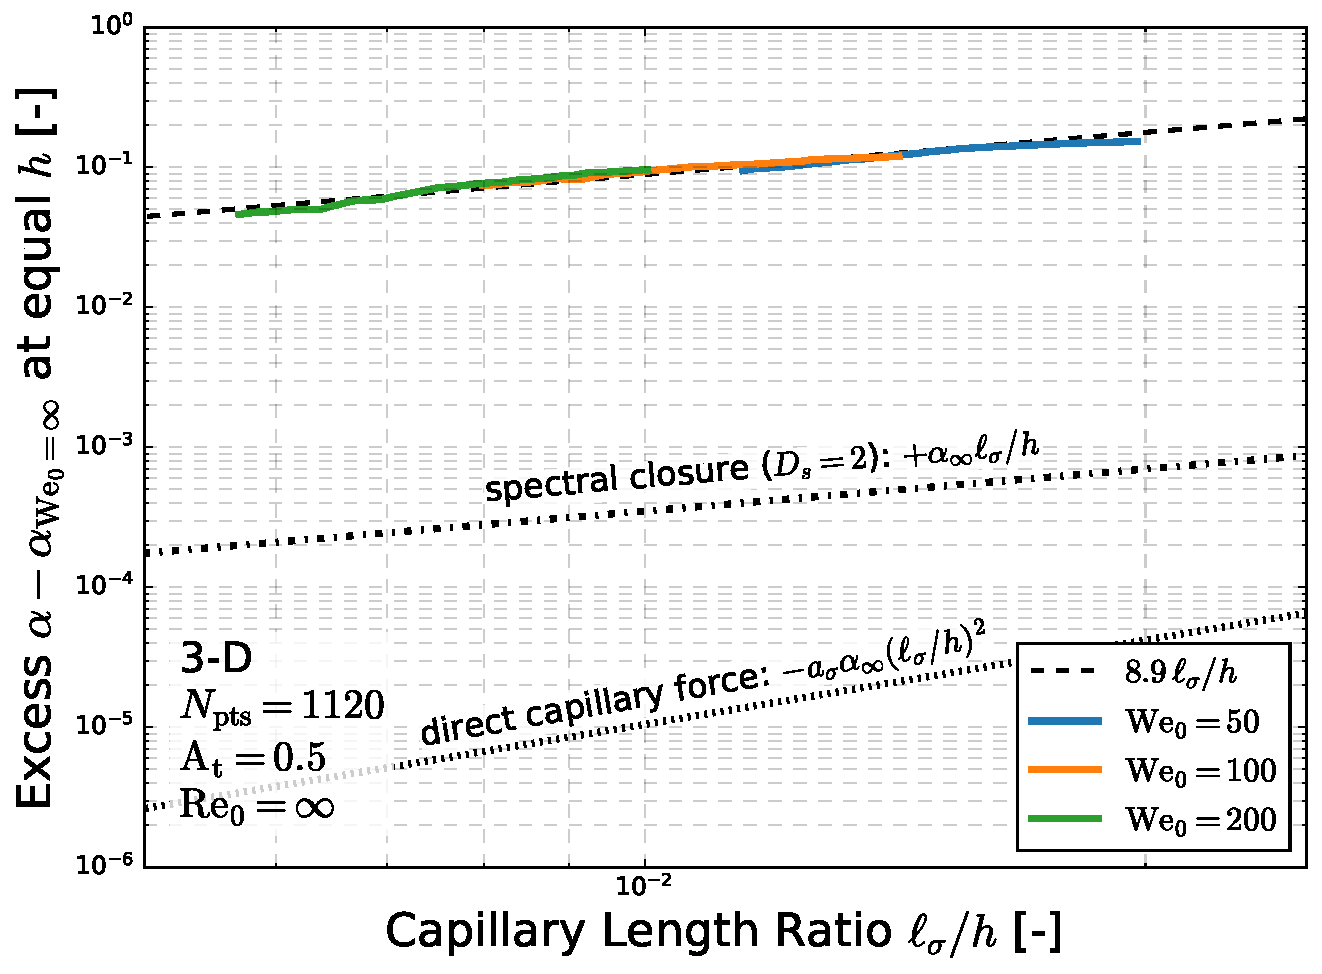
\includegraphics[width=\linewidth]{fig_excess_width}\end{minipage}\hfill
  \begin{minipage}[t]{0.49\textwidth}\raggedright (\textit{b})\\[-2pt]
    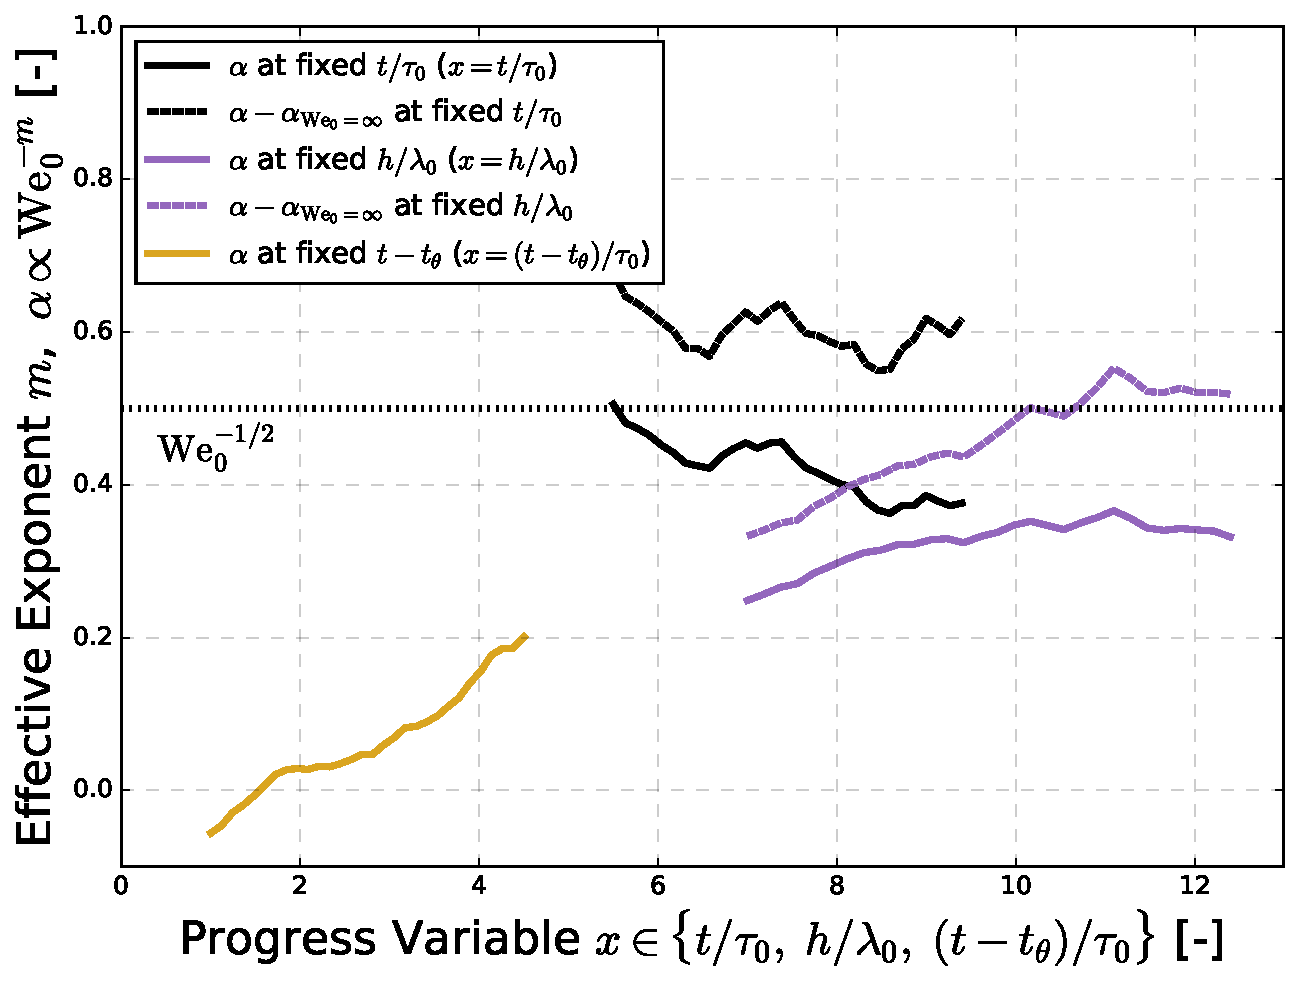
\includegraphics[width=\linewidth]{fig_We_exponent}\end{minipage}
  \caption{(\textit{a}) Excess $\alpha - \alpha_{\We = \infty}$ at equal $h$ against $\lls/h$ for $7 \le h/\lambda_0 \le 12.5$, with the fit (\ref{eq:fit}), the spectral closure (\ref{eq:closure}) with $D_s = 2$, and the magnitude of the direct correction (\ref{eq:direct}) with $a_\sigma \approx 3$. (\textit{b}) Effective exponent $m$ in $\alpha \propto \We^{-m}$ over $\We = 50$, $100$, $200$, for $\alpha$ and for $\alpha - \alpha_{\We = \infty}$ at fixed $t/\tau_0$ and at fixed $h/\lambda_0$, and for $\alpha$ at fixed $t - t_\theta$; $x$ is the corresponding progress variable.}
  \label{fig:excess}
\end{figure}

At fixed $h/\lambda_0$, the effective exponent of $\alpha$ itself is only $0.25$--$0.37$, because $\alpha$ includes $\alpha_\infty$, and at fixed time since the transition it rises from about zero to $0.2$ (figure~\ref{fig:excess}\textit{b}). The direct capillary term is negligible over the whole late-time range: the capillary group falls below $10^{-2}$ after the transition and is $(1.5$--$3.2) \times 10^{-4}$ at the end of the simulations (figure~\ref{fig:theory}\textit{a}). The capillary length is comparable to the grid spacing. With $\lambda_0 \approx 1.02$\,cm and $\Delta x \approx 0.114$\,cm, $\lls/\Delta x = 1.26$, $0.89$ and $0.63$ for $\We = 50$, $100$ and $200$, and the late-time effect of surface tension is nevertheless organised by $\lls$; the limit of drop breakup at the grid scale in these simulations is analysed by \citet{Walker2027_2}.

The mid-plane mass flux indicates where the indirect effect resides (\S\,S6 of the supplementary material). Without surface tension, the shape factor $R_f$ settles at $8.0$, the value for a linear profile, and with surface tension at $9.7$--$10.7$, above the self-similar range. Writing $\avg{\rho' w'}_0 = -C_r \rho_{\rm rms} w_{\rm rms}$, as in CCM04, with $\rho_{\rm rms} = (\Delta \rho/2)(1 - \theta_0)^{1/2}$ on the mid-plane and $\mathrm{Fr}_0^2 = w_{\rm rms}^2/\At g h$, the definition of $R_f$ gives $\alpha = (R_f^2/16) \, C_r^2 \,(1 - \theta_0) \, \mathrm{Fr}_0^2$. Averaged over $8 \le t/\tau_0 \le 9.4$, the factor $3.84$ in $\alpha$ between $\We = 50$ and $\We = \infty$ splits as $1.76$ from $R_f^2$, $1.49$ from the purity $1 - \theta_0$ and $1.46$ from $C_r^2 \mathrm{Fr}_0^2$, whereas the CCM04 closure, $\alpha \propto (1 - \theta_0)^{3/2}$, gives $1.82$. Between $\We = \infty$ and the miscible case, the same closure predicts $8.8$ for a factor of $1.51$, so the purity alone overpredicts the difference between miscible and immiscible growth. Surface tension therefore raises $\alpha$ through the shape factor, the purity and $C_r \mathrm{Fr}_0$ together, and these are the indirect effect required in \S\,\ref{sec:relax}. The energy budget constrains the sign in the same way: the surface energy lowers $\alpha$, so an increase with $\sigma$ must come from a smaller dissipated fraction or from a change in the profile shape.

%=====================================================================
\section{Conclusions}\label{sec:conclusions}

Complete self-similarity leaves no dimensionless group that contains $\sigma$, so surface tension can change the late-time growth parameter of immiscible RT turbulence only through corrections in $\lls/h$. In the self-similar moment equations extended to immiscible fluids, the direct capillary term is the inverse instantaneous Weber number; it reduces $\alpha$ and scales as $\We^{-1}$. The moment balance with fixed constants relaxes approximately as $h^{-40}$, so the observed increase of $\alpha$, which decays only as $h^{-1}$, requires an indirect effect of surface tension on the flow structure. A correction linear in $\lls/h$ is the form that this effect takes in simulations: compared at equal mixing width, $\alpha - \alpha_{\We = \infty} \approx 8.9 \, \lls/h$, which is a $\We^{-1/2}$ dependence at fixed $h/\lambda_0$ and vanishes as $h/\lls \rightarrowtriangle \infty$. A power law in $\We$ extracted at fixed time has an exponent that drifts with the time of comparison. A spectral closure in which surface tension sets the inner cut-off of a smooth interface reproduces the exponent and the sign but not the magnitude, and the mass-flux decomposition divides the effect among the shape factor $R_f$, the purity and $C_r \mathrm{Fr}_0$, while the purity alone overpredicts the difference between miscible and immiscible growth. The coefficient $K$ remains to be determined by a closure for the profile constants $\chi_0$ and $\hat D$ in the presence of surface tension.

\backsection[Supplementary data]{\label{SupMat}Supplementary material is available at \url{https://doi.org/} \dots.}

\backsection[Acknowledgements]{This report was prepared as an account of work sponsored by an agency of the United States Government. Neither the U.S. Government nor any agency thereof, nor any of their employees, makes any warranty, express or implied, or assumes any legal liability or responsibility for the accuracy, completeness, or usefulness of any information, apparatus, product, or process disclosed, or represents that its use would not infringe privately owned rights. Reference herein to any specific commercial product, process, or service by trade name, trademark, manufacturer, or otherwise does not necessarily constitute or imply its endorsement, recommendation, or favoring by the U.S. Government or any agency thereof. The views and opinions of authors expressed herein do not necessarily state or reflect those of the U.S. Government or any agency thereof.
}

\backsection[Funding]{This material is based upon work supported by the U.S. Department of Energy, Office of Science, Office of Advanced Scientific Computing Research, Department of Energy Computational Science Graduate Fellowship under Award Number DE-SC0024386.}
% This work was performed under the auspices of the U.S. Department of Energy by Lawrence Livermore National Laboratory under Contract DE-AC52-07NA27344. This article has been assigned an LLNL document release number (LLNL-XXX-XXXXXXX).

\backsection[Declaration of interests]{%A Competing Interests statement is now mandatory in the manuscript PDF. Please note that if there are no conflicts of interest, the declaration in your PDF should read as follows: {\bf Declaration of Interests}.
The authors report no conflict of interest.}

\backsection[Data availability statement]{The data that support the findings of this study are openly available on GitHub at \url{https://github.com/mw6136/alpha-theory}.}

\backsection[Author ORCIDs]{ M. D. Walker, https://orcid.org/0000-0002-4765-6539; S. S. Nixon, https://orcid.org/0009-0003-5313-9081}

\backsection[Author contributions]{M. D. Walker: Methodology, Formal analysis, Investigation, Software, Data curation, Writing -- original draft. S. S. Nixon: Conceptualization, Methodology, Formal analysis, Writing -- review \& editing.}

\bibliographystyle{jfm}
\bibliography{jfm}

\end{document}